%!TEX TS-program = xelatex
%!TEX encoding = UTF-8 Unicode
% Awesome CV LaTeX Template for CV/Resume
%
% This template has been downloaded from:
% https://github.com/posquit0/Awesome-CV
%
% Author:
% Claud D. Park <posquit0.bj@gmail.com>
% http://www.posquit0.com
%
% Template license:
% CC BY-SA 4.0 (https://creativecommons.org/licenses/by-sa/4.0/)
%


%-------------------------------------------------------------------------------
% CONFIGURATIONS
%-------------------------------------------------------------------------------
% A4 paper size by default, use 'letterpaper' for US letter
\documentclass[11pt, a4paper]{awesome-cv}

% Configure page margins with geometry
\geometry{left=1.4cm, top=.8cm, right=1.4cm, bottom=1.8cm, footskip=.5cm}

% Specify the location of the included fonts
\fontdir[fonts/]

% Color for highlights
% Awesome Colors: awesome-emerald, awesome-skyblue, awesome-red, awesome-pink, awesome-orange
%                 awesome-nephritis, awesome-concrete, awesome-darknight
\colorlet{awesome}{awesome-red}
% Uncomment if you would like to specify your own color
% \definecolor{awesome}{HTML}{CA63A8}

% Colors for text
% Uncomment if you would like to specify your own color
% \definecolor{darktext}{HTML}{414141}
% \definecolor{text}{HTML}{333333}
% \definecolor{graytext}{HTML}{5D5D5D}
% \definecolor{lighttext}{HTML}{999999}

% Set false if you don't want to highlight section with awesome color
\setbool{acvSectionColorHighlight}{true}

% If you would like to change the social information separator from a pipe (|) to something else
\renewcommand{\acvHeaderSocialSep}{\quad\textbar\quad}


%-------------------------------------------------------------------------------
%	PERSONAL INFORMATION
%	Comment any of the lines below if they are not required
%-------------------------------------------------------------------------------
% Available options: circle|rectangle,edge/noedge,left/right
% \photo{./examples/profile.png}
\name{Claud D.}{Park}
\position{Software Architect{\enskip\cdotp\enskip}Security Expert}
\address{42-8, Bangbae-ro 15-gil, Seocho-gu, Seoul, 00681, Rep. of KOREA}

\mobile{(+82) 10-9030-1843}
\email{posquit0.bj@gmail.com}
\homepage{www.posquit0.com}
\github{posquit0}
\linkedin{posquit0}
% \gitlab{gitlab-id}
% \stackoverflow{SO-id}{SO-name}
% \twitter{@twit}
% \skype{skype-id}
% \reddit{reddit-id}
% \medium{madium-id}
% \googlescholar{googlescholar-id}{name-to-display}
%% \firstname and \lastname will be used
% \googlescholar{googlescholar-id}{}
% \extrainfo{extra informations}

\quote{``Be the change that you want to see in the world."}

%-------------------------------------------------------------------------------
%	BIBLIOGRAPHY
%-------------------------------------------------------------------------------
\addbibresource{cv/references.bib}

%-------------------------------------------------------------------------------
\begin{document}

% Print the header with above personal informations
% Give optional argument to change alignment(C: center, L: left, R: right)
\makecvheader

% Print the footer with 3 arguments(<left>, <center>, <right>)
% Leave any of these blank if they are not needed
\makecvfooter
  {\today}
  {Claud D. Park~~~·~~~Curriculum Vitae}
  {\thepage}


%-------------------------------------------------------------------------------
%	CV/RESUME CONTENT
%	Each section is imported separately, open each file in turn to modify content
%-------------------------------------------------------------------------------
%!TEX root = ../cv.tex
% -*- root: ../cv.tex -*-

%-------------------------------------------------------------------------------
% SECTION TITLE
%-------------------------------------------------------------------------------
\cvsection{Education}


%-------------------------------------------------------------------------------
% CONTENT
%-------------------------------------------------------------------------------
\begin{cventries}

%---------------------------------------------------------
  \cventry
    {컴퓨터정보산업공학과 공학사} % Degree
    {연세대학교} % Institution
    {서울특별시} % Location
    {2001.03 - 2006.02} % Date(s)
    {}

%---------------------------------------------------------

  \cventry
    {컴퓨터과학과 공학석사} % Degree
    {연세대학교} % Institution
    {서울특별시} % Location
    {2006.03 - 2008.02} % Date(s)
    {
      % \begin{cvitems} % Description(s) bullet points
      %   \item {Got a Chun Shin-Il Scholarship which is given to promising students in CSE Dept.}
      % \end{cvitems}
    }

  \cventry
    {컴퓨터과학과 공학박사} % Degree
    {연세대학교} % Institution
    {서울특별시} % Location
    {2008.03 - 2016.08} % Date(s)
    {
      % \begin{cvitems} % Description(s) bullet points
      %   \item {Got a Chun Shin-Il Scholarship which is given to promising students in CSE Dept.}
      % \end{cvitems}
    }
\end{cventries}

%!TEX root = ../cv.tex
% -*- root: ../cv.tex -*-

%-------------------------------------------------------------------------------
%	SECTION TITLE
%-------------------------------------------------------------------------------
\cvsection{Skills}


%-------------------------------------------------------------------------------
%	CONTENT
%-------------------------------------------------------------------------------
\begin{cvskills}

%---------------------------------------------------------
  \cvskill
    {Deep Learning / Computer Vision} % Category
    {TensorFlow, Keras, OpenCV} % Skills

%---------------------------------------------------------
  \cvskill
    {Programming} % Category
    {C/C++, JAVA, Python, QML, C\#} % Skills

%---------------------------------------------------------
  \cvskill
    {SW Frameworks} % Category
    {Qt/QML, OpenFrameworks, Processing, Arduino, Android, WPF} % Skills

%---------------------------------------------------------
  \cvskill
    {Languages} % Category
    {Korean, English} % Skills

%---------------------------------------------------------
\end{cvskills}

%!TEX root = ../cv.tex
% -*- root: ../cv.tex -*-

%-------------------------------------------------------------------------------
%	SECTION TITLE
%-------------------------------------------------------------------------------
\cvsection{Experience}


%-------------------------------------------------------------------------------
%	CONTENT
%-------------------------------------------------------------------------------
\begin{cventries}
%---------------------------------------------------------
  \cventry
    {Deep Learning} % Job title
    {} % Organization
    {} % Location
    {Level: B+} % Date(s)
    {
      \begin{cvitems} % Description(s) of tasks/responsibilities
        \item {Research on Deep Learning based Object Detection for Defect Detection/Inspection}
        \item {Develop on Steering Wheel Classification Algorithm}
      \end{cvitems}
    }

%---------------------------------------------------------
  \cventry
    {Computer Vision and Pattern Recognition} % Job title
    {} % Organization
    {} % Location
    {Level: B+} % Date(s)
    {
      \begin{cvitems} % Description(s) of tasks/responsibilities
        \item {Develop for Mobile Augmented Reality using Local Feature Tracking \\
               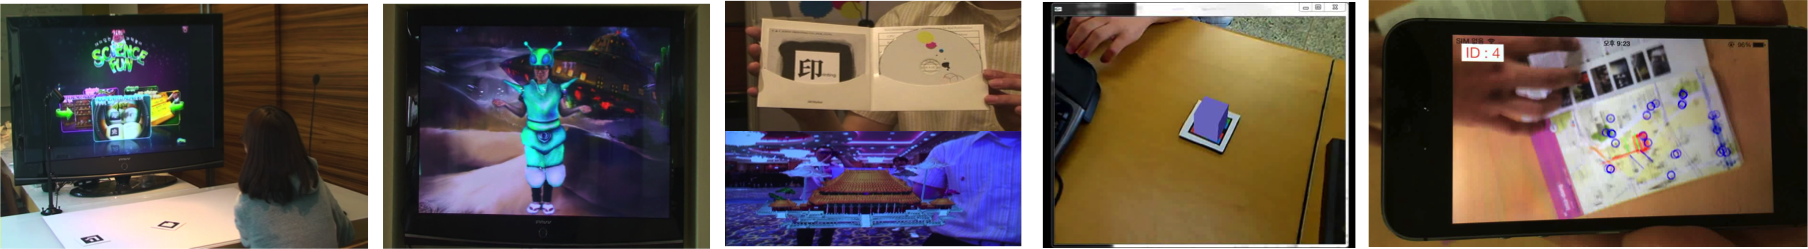
\includegraphics[width=\linewidth]{resources/ar.png} }
          \begin{itemize}
            \item {Develop a feature point filtering algorithm for high performance and speed}
          \end{itemize}
        \item {Research on Recognizing Bare Hands using Depth Camera \\
               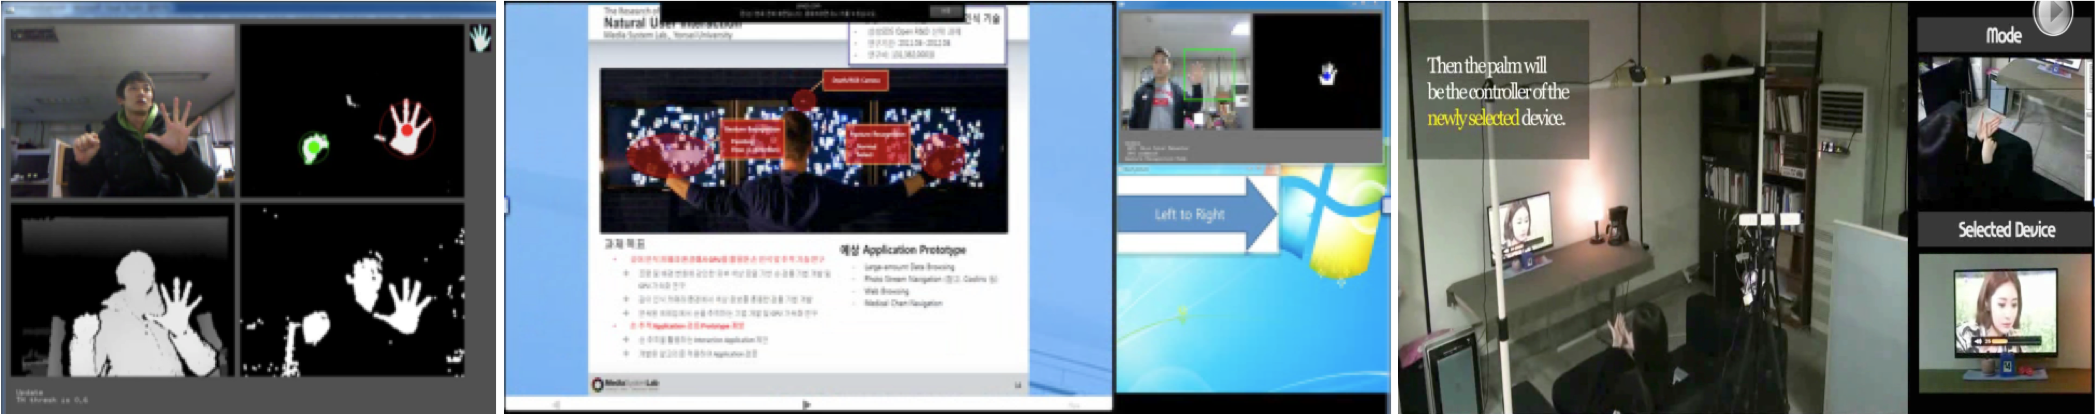
\includegraphics[width=\linewidth]{resources/hand.png} }
        \item {Spoke/Steering Wheel Region Tracking for Driver Status Monitoring}
      \end{cvitems}
    }

%---------------------------------------------------------
  \cventry
    {Device Fast Prototyping} % Job title
    {} % Organization
    {} % Location
    {Level: A+} % Date(s)
    {
      \begin{cvitems} % Description(s) of tasks/responsibilities
        \item {Developing Spatial AR Environment using $360^{\circ}$ Steerable Projector \\
          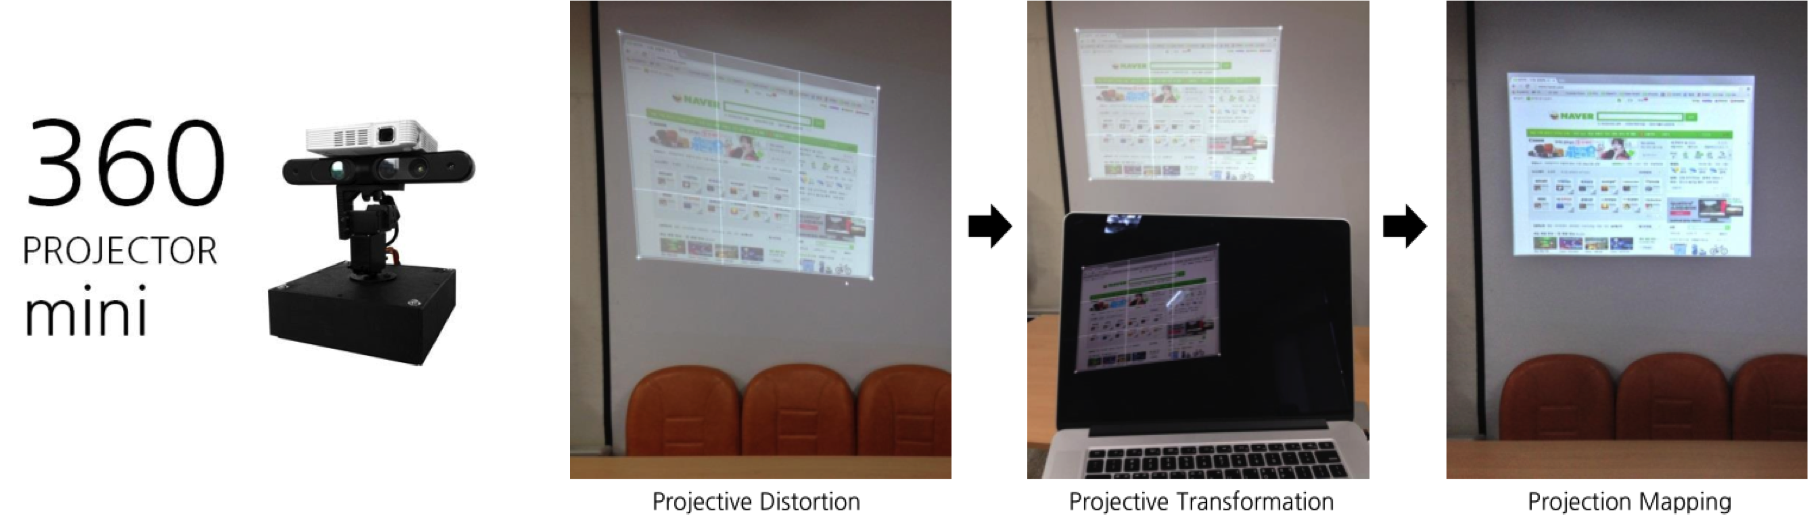
\includegraphics[width=\linewidth]{resources/pervasiveAR.png}
          \begin{itemize}
              \item {Pico Projector, Small Depth Camera, Arduino based Pan-Tilt Motor System}
              \item {Research a computer vision based projecting image rectification algorithm for pan-tilt projector}
          \end{itemize}
        }
        \item {Pen-type Interface which Augments Information on the Surface \\
          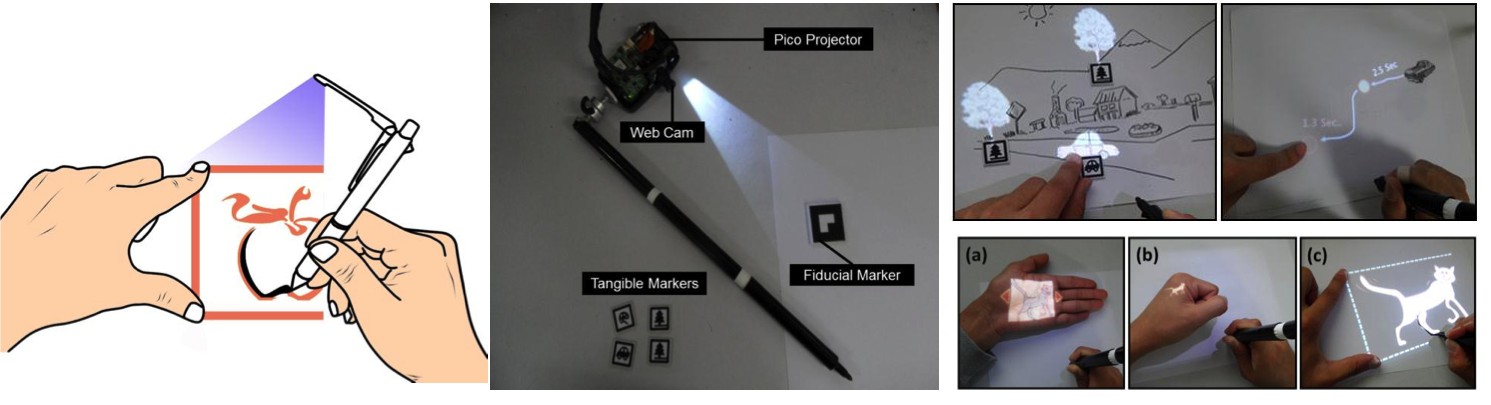
\includegraphics[width=\linewidth, height=40mm]{resources/augpen.png}
          \begin{itemize}
            \item {Pico Projector, Small Web Camera, Fiducial Marker}
            \item {Research on Interating Technology with 2D Contents and Bare Hand}
          \end{itemize}
        }
        \item {Sensor-based Gestural Interfaces \\
          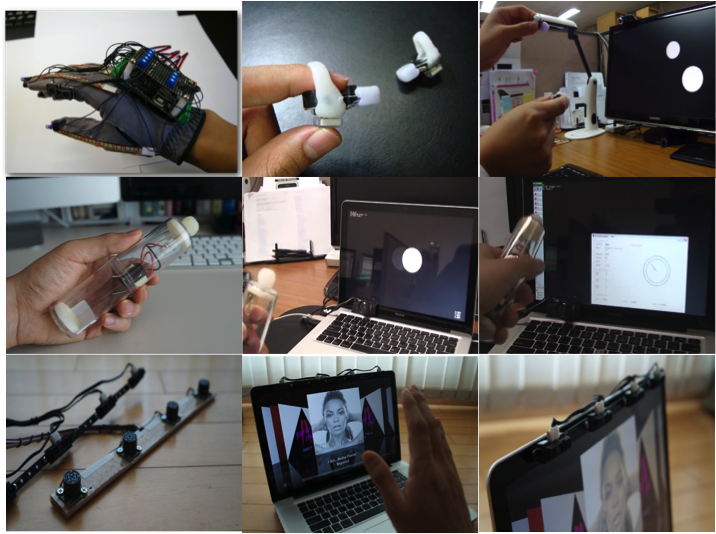
\includegraphics[width=\linewidth]{resources/gesturedevices.png}
          \begin{itemize}
            \item {Developing Various Types of Sensor Interfaces to Recognize Hand Interaction}
            \item {Developing Gesture Interface using IR Blob, Flex Sensor, Gyro Sensor, Lidar Sensor, etc}
          \end{itemize}
        }
      \end{cvitems}
    }
\end{cventries}

%-------------------------------------------------------------------------------
%	SECTION TITLE
%-------------------------------------------------------------------------------
\cvsection{Extracurricular Activity}


%-------------------------------------------------------------------------------
%	CONTENT
%-------------------------------------------------------------------------------
\begin{cventries}

%---------------------------------------------------------
  \cventry
    {Core Member} % Affiliation/role
    {B10S (B1t 0n the Security, Underground hacker team)} % Organization/group
    {S.Korea} % Location
    {Nov. 2011 - PRESENT} % Date(s)
    {
      \begin{cvitems} % Description(s) of experience/contributions/knowledge
        \item {Gained expertise in penetration testing areas, especially targeted on web application and software.}
        \item {Participated on a lot of hacking competition and won a good award.}
        \item {Held several hacking competitions non-profit, just for fun.}
      \end{cvitems}
    }

%---------------------------------------------------------
  \cventry
    {Member} % Affiliation/role
    {WiseGuys (Hacking \& Security research group)} % Organization/group
    {S.Korea} % Location
    {Jun. 2012 - PRESENT} % Date(s)
    {
      \begin{cvitems} % Description(s) of experience/contributions/knowledge
        \item {Gained expertise in hardware hacking areas from penetration testing on several devices including wireless router, smartphone, CCTV and set-top box.}
        \item {Trained wannabe hacker about hacking technique from basic to advanced and ethics for white hackers by hosting annual Hacking Camp.}
      \end{cvitems}
    }

%---------------------------------------------------------
  \cventry
    {Core Member \& President at 2013} % Affiliation/role
    {PoApper (Developers' Network of POSTECH)} % Organization/group
    {Pohang, S.Korea} % Location
    {Jun. 2010 - Jun. 2017} % Date(s)
    {
      \begin{cvitems} % Description(s) of experience/contributions/knowledge
        \item {Reformed the society focusing on software engineering and building network on and off campus.}
        \item {Proposed various marketing and network activities to raise awareness.}
      \end{cvitems}
    }

%---------------------------------------------------------
  \cventry
    {Member} % Affiliation/role
    {PLUS (Laboratory for UNIX Security in POSTECH)} % Organization/group
    {Pohang, S.Korea} % Location
    {Sep. 2010 - Oct. 2011} % Date(s)
    {
      \begin{cvitems} % Description(s) of experience/contributions/knowledge
        \item {Gained expertise in hacking \& security areas, especially about internal of operating system based on UNIX and several exploit techniques.}
        \item {Participated on several hacking competition and won a good award.}
        \item {Conducted periodic security checks on overall IT system as a member of POSTECH CERT.}
        \item {Conducted penetration testing commissioned by national agency and corporation.}
      \end{cvitems}
    }

%---------------------------------------------------------
  \cventry
    {Member} % Affiliation/role
    {MSSA (Management Strategy Club of POSTECH)} % Organization/group
    {Pohang, S.Korea} % Location
    {Sep. 2013 - Jun. 2017} % Date(s)
    {
      \begin{cvitems} % Description(s) of experience/contributions/knowledge
        \item {Gained knowledge about several business field like Management, Strategy, Financial and marketing from group study.}
        \item {Gained expertise in business strategy areas and inisght for various industry from weekly industry analysis session.}
      \end{cvitems}
    }

%---------------------------------------------------------
\end{cventries}

%-------------------------------------------------------------------------------
%	SECTION TITLE
%-------------------------------------------------------------------------------
\cvsection{Honors \& Awards}


%-------------------------------------------------------------------------------
%	SUBSECTION TITLE
%-------------------------------------------------------------------------------
\cvsubsection{International}


%-------------------------------------------------------------------------------
%	CONTENT
%-------------------------------------------------------------------------------
\begin{cvhonors}

%---------------------------------------------------------
  \cvhonor
    {Finalist} % Award
    {DEFCON 26th CTF Hacking Competition World Final} % Event
    {Las Vegas, U.S.A} % Location
    {2018} % Date(s)

%---------------------------------------------------------
  \cvhonor
    {Finalist} % Award
    {DEFCON 25th CTF Hacking Competition World Final} % Event
    {Las Vegas, U.S.A} % Location
    {2017} % Date(s)

%---------------------------------------------------------
  \cvhonor
    {Finalist} % Award
    {DEFCON 22nd CTF Hacking Competition World Final} % Event
    {Las Vegas, U.S.A} % Location
    {2014} % Date(s)

%---------------------------------------------------------
  \cvhonor
    {Finalist} % Award
    {DEFCON 21st CTF Hacking Competition World Final} % Event
    {Las Vegas, U.S.A} % Location
    {2013} % Date(s)

%---------------------------------------------------------
  \cvhonor
    {Finalist} % Award
    {DEFCON 19th CTF Hacking Competition World Final} % Event
    {Las Vegas, U.S.A} % Location
    {2011} % Date(s)

%---------------------------------------------------------
\end{cvhonors}


%-------------------------------------------------------------------------------
%	SUBSECTION TITLE
%-------------------------------------------------------------------------------
\cvsubsection{Domestic}


%-------------------------------------------------------------------------------
%	CONTENT
%-------------------------------------------------------------------------------
\begin{cvhonors}

%---------------------------------------------------------
  \cvhonor
    {3rd Place} % Award
    {WITHCON Hacking Competition Final} % Event
    {Seoul, S.Korea} % Location
    {2015} % Date(s)

%---------------------------------------------------------
  \cvhonor
    {Silver Prize} % Award
    {KISA HDCON Hacking Competition Final} % Event
    {Seoul, S.Korea} % Location
    {2017} % Date(s)

%---------------------------------------------------------
  \cvhonor
    {Silver Prize} % Award
    {KISA HDCON Hacking Competition Final} % Event
    {Seoul, S.Korea} % Location
    {2013} % Date(s)

%---------------------------------------------------------
\end{cvhonors}

%!TEX root = ../cv.tex
% -*- root: ../cv.tex -*-

%-------------------------------------------------------------------------------
% SECTION TITLE
%-------------------------------------------------------------------------------
\cvsection{Presentation}


%-------------------------------------------------------------------------------
% CONTENT
%-------------------------------------------------------------------------------
\begin{cventries}

%---------------------------------------------------------
  \cventry
    {차세대 스마트 센서 융합 기술 세미나} % Role
    {웨어러블 환경에서의 모션 인식: 모션센서 기반의 웨어러블 제어 기술} % Event
    {한국미래기술교육연구원 (\href{http://nvyt.kecft.or.kr/bbs/bbsView.php?id=146&code=bbs_schedule&bbs_id=2}{Link})} % Location
    {27, Mar. 2014} % Date(s)
    {}

%---------------------------------------------------------
  \cventry
  % • 2013.10.17  eBiz 연구회, “모션인식 2.0: 키넥트 이후의 모션인식 기술”
    {eBiz 연구회 정기 세미나} % Role
    {모션인식 2.0} % Event
    {eBiz 연구회 (\href{http://www.dure.net/SIG.html}{Link})} % Location
    {17, Oct. 2013} % Date(s)
    {}

%---------------------------------------------------------
  \cventry
  % • 2013.09.27  K모바일, 웨어러블 컴퓨터 비즈니스 레볼루션 2014, “웨어러블 시대의 킬러앱은? – 웨어러블 컴퓨터 서비스 시나리오”
    {웨어러블 컴퓨터 비즈니스 레볼루션 2014} % Role
    {웨어러블 시대의 킬러앱은?: 웨어러블 컴퓨터 서비스 시나리오} % Event
    {K모바일} % Location
    {27, Sep. 2013} % Date(s)
    {}

%---------------------------------------------------------
  \cventry
  % • 2013.07.16  ETRI 사내 세미나, “모션인식 2.0: 키넥트 이후의 모션인식 기술”
    {ETRI 사내 세미나} % Role
    {모션인식 2.0: 키넥트 이후의 모션인식 기술} % Event
    {ETRI} % Location
    {16, Jul. 2013} % Date(s)
    {}

%---------------------------------------------------------
  \cventry
  % • 2013.07.11  K모바일, 코리아 네추럴UI/UX 세미나, “모션인식 2.0: 키넥트 이후의 모션인식 기술”
    {코리아 네추럴UI/UX 세미나} % Role
    {모션인식 2.0: 키넥트 이후의 모션인식 기술} % Event
    {K모바일} % Location
    {11, Jul. 2013} % Date(s)
    {(SlideShare 2014년도 상위 5\% 열람 기록)}

%---------------------------------------------------------
  \cventry
  % • 2011.06.24  삼성SDS 사내 세미나, “Gesture Interface 기술 동향 및 전망”
    {삼성SDS 사내 세미나} % Role
    {Gesture Interface 기술 동향 및 전망} % Event
    {삼성SDS} % Location
    {24, Jun. 2011} % Date(s)
    {}
    
%---------------------------------------------------------
  \cventry
  % • 2011.01.28  K모바일 코리아 모바일 UX 컨퍼런스, “모션 인식 인터페이스 기술 동향과 전망”
    {코리아 모바일 UX 컨퍼런스} % Role
    {모션 인식 인터페이스 기술 동향과 전망} % Event
    {K모바일} % Location
    {28, Jan. 2011} % Date(s)
    {}
%---------------------------------------------------------
\end{cventries}

%%-------------------------------------------------------------------------------
%	SECTION TITLE
%-------------------------------------------------------------------------------
\cvsection{Writing}


%-------------------------------------------------------------------------------
%	CONTENT
%-------------------------------------------------------------------------------
\begin{cventries}

%---------------------------------------------------------
  \cventry
    {Founder \& Writer} % Role
    {A Guide for Developers in Start-up} % Title
    {Facebook Page} % Location
    {Jan. 2015 - PRESENT} % Date(s)
    {
      \begin{cvitems} % Description(s)
        \item {Drafted daily news for developers in Korea about IT technologies, issues about start-up.}
      \end{cvitems}
    }

%---------------------------------------------------------
\end{cventries}

%-------------------------------------------------------------------------------
%	SECTION TITLE
%-------------------------------------------------------------------------------
\cvsection{Publications}

%-------------------------------------------------------------------------------
%	SUBSECTION TITLE
%-------------------------------------------------------------------------------
\cvsubsection{Journal Articles}

\begin{refsection}
	\nocite{Khan2014Incentive}
	\nocite{Selimi2015Cloud}
	
	\newrefcontext[sorting=ydnt]
	\printbibliography[heading=none]
\end{refsection}

%-------------------------------------------------------------------------------
%	SUBSECTION TITLE
%-------------------------------------------------------------------------------
\cvsubsection{Conference Proceedings}

\begin{refsection}
    \nocite{Khan2014Prototyping}
	
	\newrefcontext[sorting=ydnt]
	\printbibliography[heading=none]
\end{refsection}

%-------------------------------------------------------------------------------
%	SECTION TITLE
%-------------------------------------------------------------------------------
\cvsection{Program Committees}


%-------------------------------------------------------------------------------
%	CONTENT
%-------------------------------------------------------------------------------
\begin{cvhonors}

%---------------------------------------------------------
  \cvhonor
    {Problem Writer} % Position
    {2016 CODEGATE Hacking Competition World Final} % Committee
    {S.Korea} % Location
    {2016} % Date(s)

%---------------------------------------------------------
  \cvhonor
    {Organizer \& Co-director} % Position
    {1st POSTECH Hackathon} % Committee
    {S.Korea} % Location
    {2013} % Date(s)

%---------------------------------------------------------
\end{cvhonors}



%-------------------------------------------------------------------------------
\end{document}
